\subsection{Intuitive Visualization, GUI and Other Functionalities}
\label{sec:gui}

\begin{comment}
(a) permit an already partially generated atlas to be input; in this case algorithm proceeds from one of the unfinished regions of the current stratification; \\
(b) start from a specified bi-tether or a specified region of the current stratification; \\
(c) change the traversal of the stratification from depth to breadth first, for any specified region of the current stratification; \\
(d) choose to only traverse specified regions of the current stratification; \\
(e) allows increased sampling refinement for specified regions. \\
(f) limits stratification to regions satisfying global assembly constraints \\
(g) extends stratification to include regions defined by active global assembly constraints.\\
\end{comment}

%(b) EASAL allows user to start sampling from an arbitrary AtlasNode through appropriate Interface class AtlasNodeSelectionWindow that allows user selecting set of active constraints for the ActiveConstraintGraph.

% The Interface class HelixMainWindow allows user to define any settings such as step size, thresholds, whether to activate any type constraints i.e. sterics, angle .. or not, to select \helix input files, to define the location where to store atlas..

%The Interface class TableSelect allows user to do changes on input \helix file such as playing with the naming, coordinates or radius of atoms or allowing which atoms to be included helix.



The \EASAL\ user interface provides the following functionalities:

\begin{itemize}
\item Selecting input molecular data. \rahul{When starting afresh,
\EASAL\ allows the user to enter molecular data in formats such as
the PDB data describing the molecular composites, 3D structure or 
the location of an existing atlas that needs further sampling. 
In the case a partially generated atlas exists, the algorithm
does not expect any new input and proceeds from one of the 
unfinished regions of the current stratification.}

\item Real-time intervention at any stage of the sampling process;
allowing the user to halt, direct, and resume the sampling process and
to access the atlas for different queries or views.

\item Visualization of the atlas, active constraint regions, and
Cartesian realizations.
\end{itemize}


The 3 visualization views are:

\begin{itemize}
\item The \aview: the stratification (\figref{fig:natlas})

\item The Cayley \pview: Cayley \chart, all or boundary
(\figref{fig:space})

\item The Cartesian \rview: instance (\figref{fig:sweep}) or
walkthrough (\figref{fig:video})
\end{itemize}



\begin{figure}[h!tbp]
\centering
\def\wid{.45\linewidth} %14
\subfigure[]{
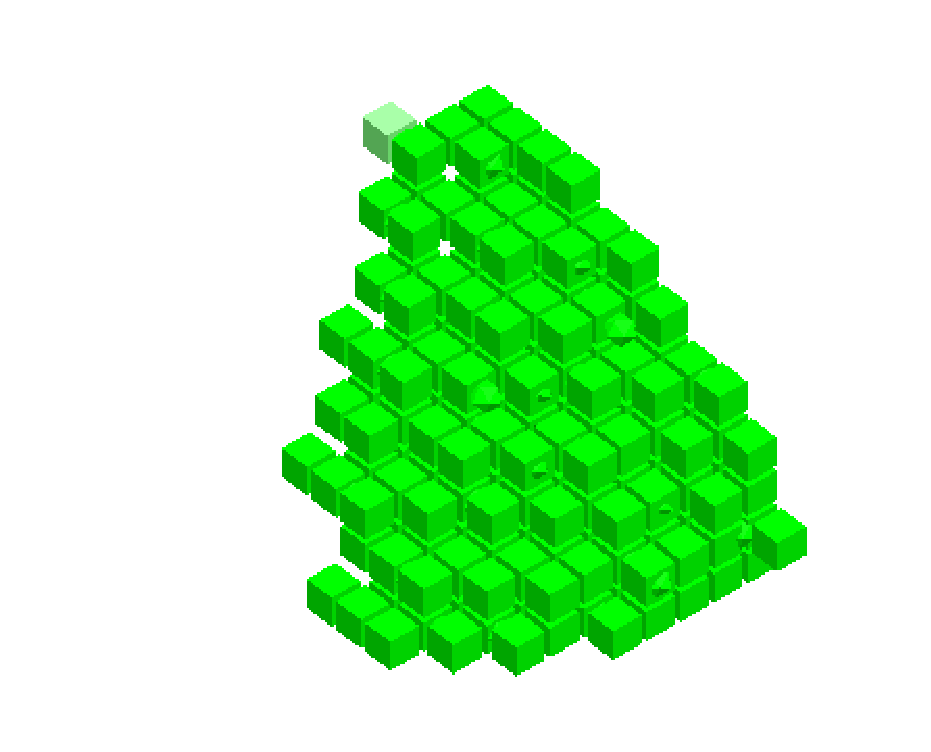
\epsfig{file = \fig/toy/108529spaceview.eps, width=0.35\linewidth}
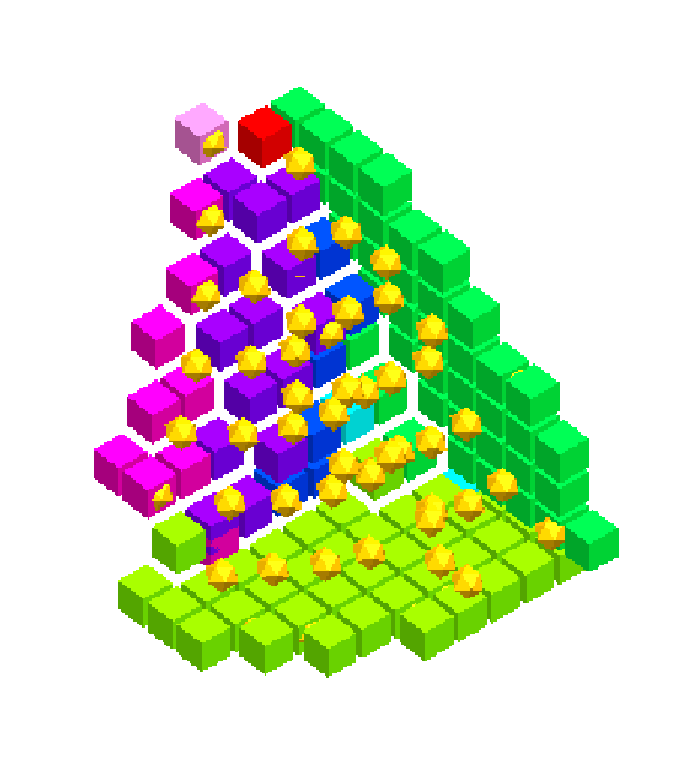
\epsfig{file = \fig/toy/108529spaceboundaries.eps, width=0.26\linewidth}
\label{fig:space}
}
\subfigure[]{
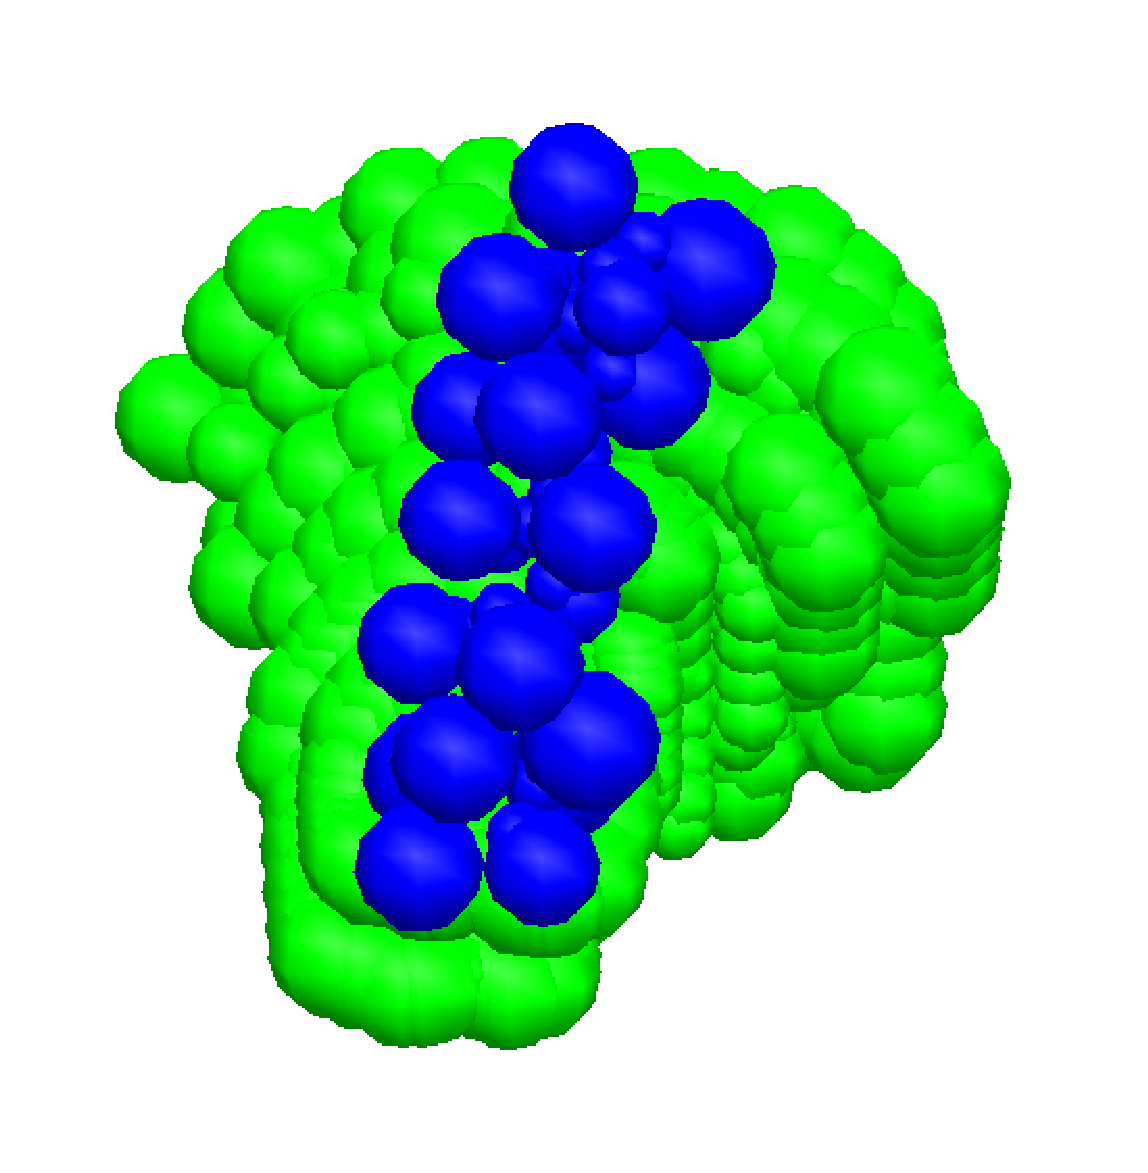
\epsfig{file = \fig/toy/108529sweepinterior.eps, width=0.3\linewidth}
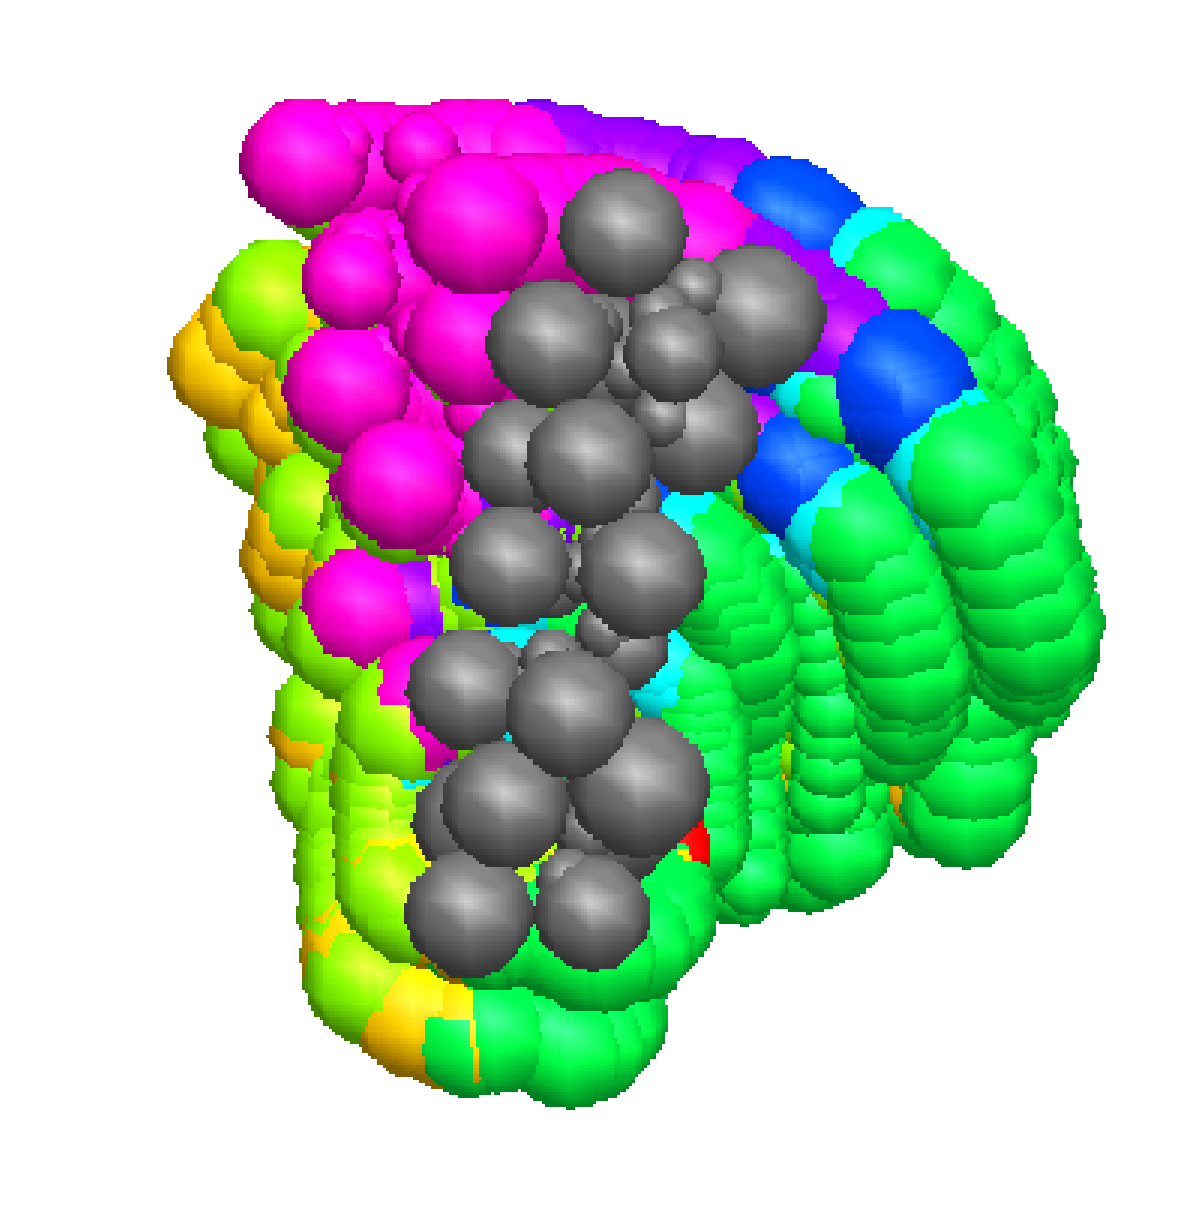
\epsfig{file = \fig/toy/108529sweepboundaries.eps,width=0.3\linewidth}
\label{fig:sweep}
}
\label{fig:spaceandsweep}
\caption[The various views of a single node chosen from the
\atlas.]{Views of a node chosen from the \atlas. (a) Cayley points in
the Cayley chart view, all versus boundary. (b) Cartesian sweep view,
all versus boundary.}
\end{figure}


The \aview\ shows the atlas as it is being built, as a tree of nodes
each representing a \cgraph. A spring-repulsion algorithm yields a
spacious layout for initial and small atlas views. \rahul{Selecting a node 
prunes the view to ancestors and descendants of the node. Clicking
a node loads its data and centres it if it has a valid realization,
or triggers the exploration of the node.}

\rahul{
The \aview\ provides controls that allow the user to intervene
in the sampling process and guide it a different direction.
\begin{itemize}
\item The dummbbell selection dialogue allows the user to choose new
constraint pairs of a \cgraph.

\item The stop sampling button allows the user to stop the sampling process. 

\item The continue sampling button, lets the user continue sampling 
that was previously stopped.

\item Clicking the refine sampling button re-samples using half the step
size of the current step size. 

\item The breadth first search button
changes the traversal of the stratification from depth to breadth
first for any specified region of the current stratification.. 

\item The complete unfinished nodes completes the sampling of 
unfinished nodes starting from the earliest discovered node.
\end{itemize}
}



\def\wid{.3\linewidth}
\begin{figure}
\centering
\subfigure{
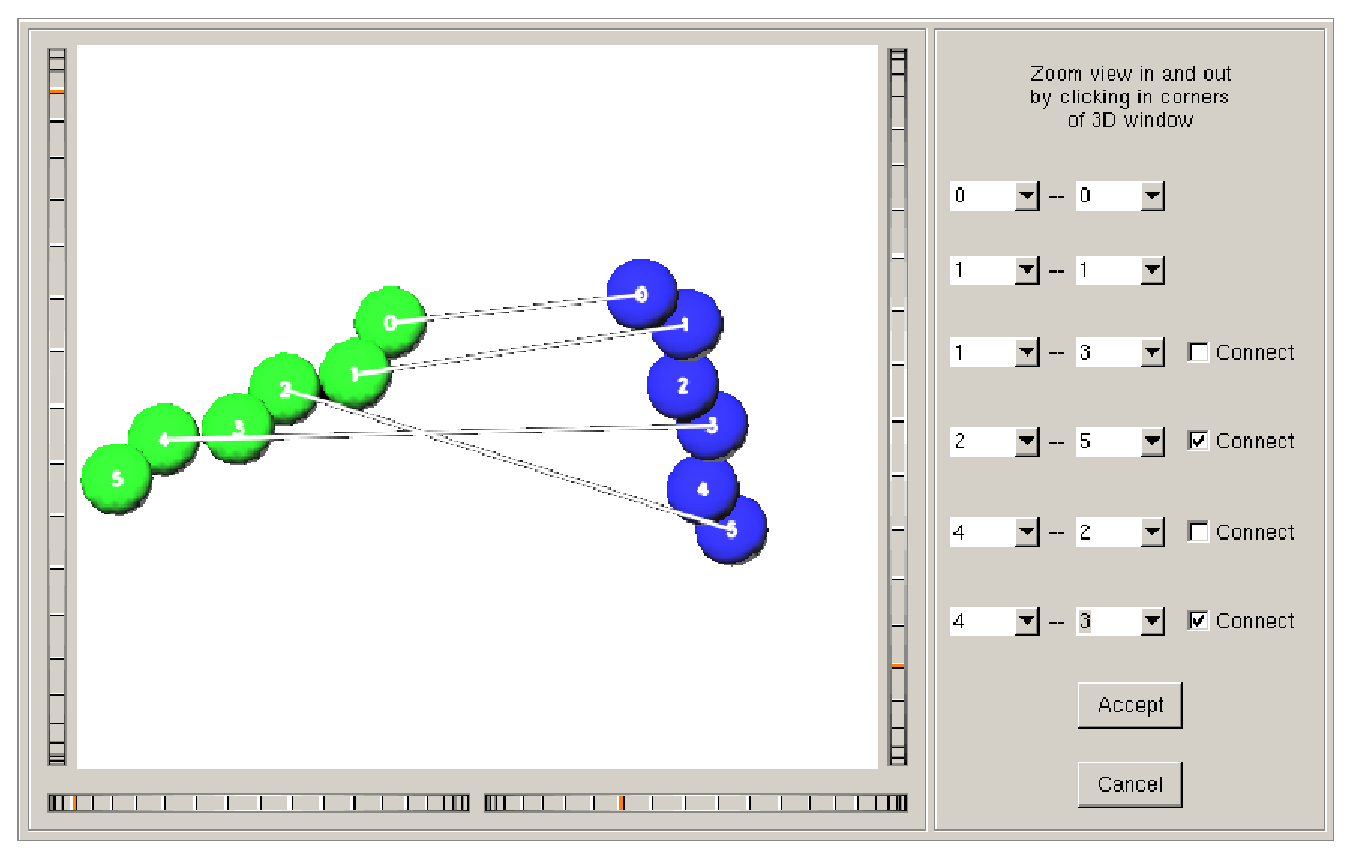
\epsfig{file=\fig/dumbellcreationwindow2.eps,width=0.5\linewidth}}
\label{fig:dumbelldialog}
\caption{The \ndialog: index choices define contact pairs.}
\end{figure}



\def\wid{.3\linewidth}
\begin{figure}
\centering
\subfigure[]{
  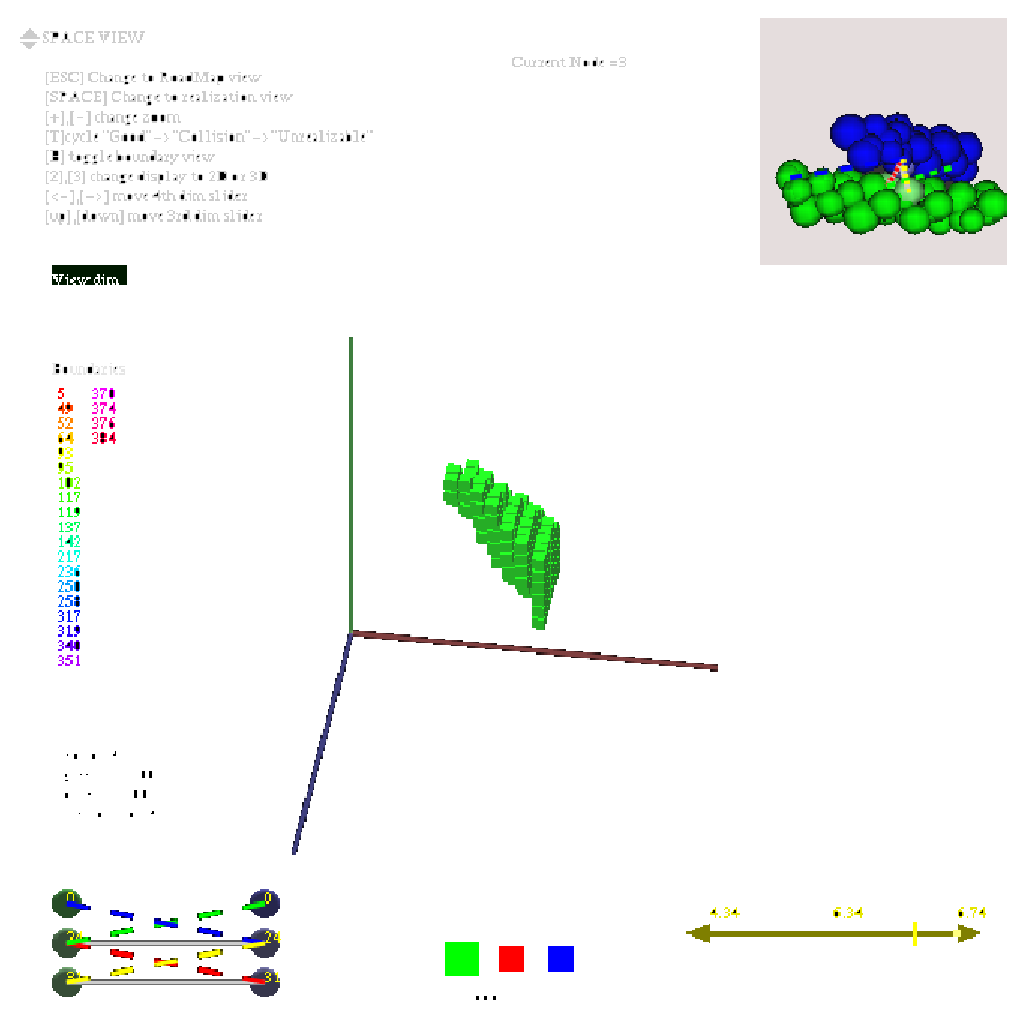
\epsfig{file=\fig/spaceview.eps,width=0.5\linewidth}
  \label{fig:spaceview}
}
\subfigure[]{
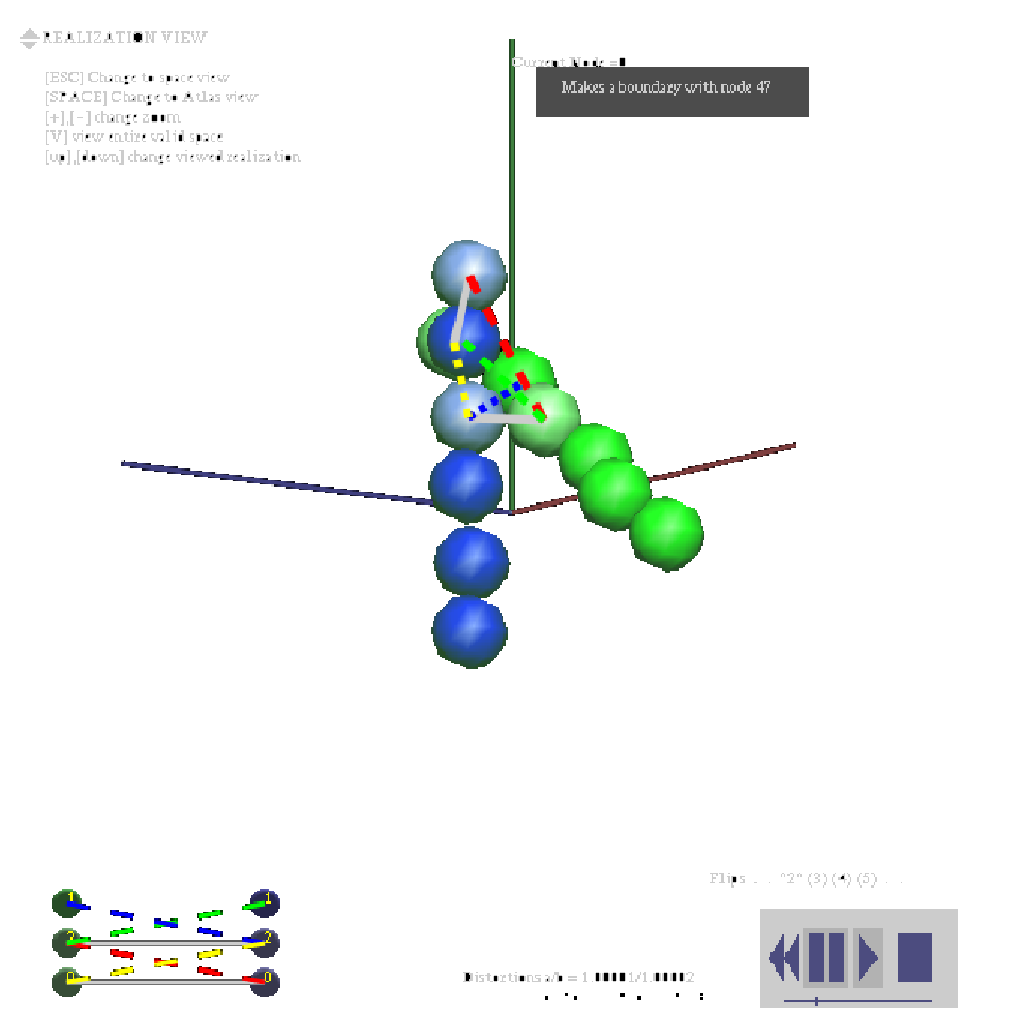
\epsfig{file=\fig/realizationview2.eps,width=0.5\linewidth}
  \label{fig:video}
}
\caption[\EASAL\ views]{
\EASAL\ views: (a) Cayley \pview: (\textit{upper right}) sample
configuration and (\textit{lower left:}) the \cgraph; (b) Cartesian
\rview\ (video): (\textit{lower left}) the \cgraph.
}
\label{fig:views}
\end{figure}



Once an \cgraph\ is sampled, the \pview\ (\figref{fig:spaceview})
shows green cubes (such that the cube size is proportional to the
step size chosen) where \param s do not result in collision.
Clicking a cube displays, in the upper right corner, a \Cr\ associated
with the \param\ values (respective Cayley point). (\EASAL\ can also
display \param s resulting in irreconcilable inter-molecular
collisions or ones that are not realizable.) For more than three
dimensions, arrow-controlled sliders select and display 3D slices. 
Since interior points are easily occluded, the third dimension can 
also be switched to a slider. The left side of the view enumerates 
newly formed lower dimensional boundaries of the active constraint 
region and enumerates color-coded boundaries.

The \rview\ (\figref{fig:video}) shows realizations with constraints
and parameters displayed as lines. Valid realization flips are shown
on the lower right side of the view. One option to view the valid
\param s in the order of detection is via `video controls' (bottom
right) with reverse, pause, play and stop options.
